
\section{Anhang}
\subsection{Trigonometrie}


$P=(\cos,\sin)$
\vspace{1mm} \hline \vspace{3 mm}

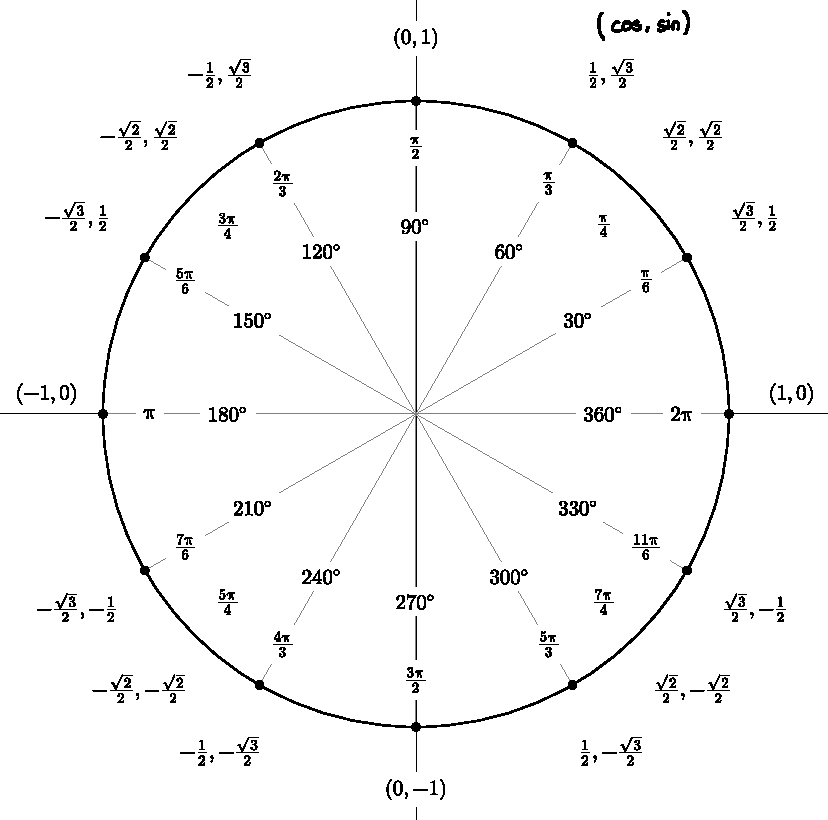
\includegraphics[scale=0.5]{build/pictures/degrees_circle.pdf} 


\begin{flushleft}

\textbf{Periodizität}
\begin{itemize}[leftmargin = *]
\item $\sin (x) & =\sin (x+2 \pi) \qquad \csc (x) = \csc (x+2 \pi)$
\item $\cos (x) & =\cos (x+2 \pi) \qquad \sec (x) = \sec (x+2 \pi)$
\item $\tan (x) & =\tan (x+\pi) \qquad \cot (x) = \cot (x+\pi)$
\item $\sin (x) = -\sin (x+\pi) \qquad \csc (x) = -\csc (x+\pi)$
\item $\cos (x) = -\cos (x+\pi) \qquad \sec (x) = -\sec (x+\pi)$
\end{itemize}

\textbf{Nullstellen}
\begin{itemize}[leftmargin = *]
\item $\sin \phi = 0$: $\phi = k\pi, \, k \in \mathbb{Z}$
\item $\cos \phi = 0$: $\phi = \frac{\pi}{2} + k\pi, \, k \in \mathbb{Z}$
\item $\tan \phi= 0$: $\phi = k\pi, \, k \in \mathbb{Z}$
\end{itemize}


\textbf{Parität}
\begin{itemize}[leftmargin = *]
 \item $\sin(-\alpha) = - \sin(\alpha) \quad \cos(-\alpha) = \cos(\alpha)$
 \item $\tan(-\alpha) = - \tan(\alpha) \quad \cot(-\alpha) = - \cot(\alpha)$
\end{itemize}

\textbf{Ergänzung}
\begin{itemize}[leftmargin = *]
 \item $\sin(\pi - \alpha) = \sin(\alpha) \quad \cos(\pi - \alpha) = - \cos(\alpha)$
 \item $\tan(\pi - \alpha) = -\tan(\alpha) \quad \cot(\pi - \alpha) = - \cot(\alpha)$
\end{itemize}


\textbf{Komplemente}
\begin{itemize}[leftmargin = *]
 \item $\sin(\pi/2 - \alpha) = \cos(\alpha) \quad \cos(\pi/2 - \alpha) = \sin(\alpha)$
 \item $\tan(\pi/2 - \alpha) = -\tan(\alpha) \quad \cot(\pi/2 - \alpha) = -\cot(\alpha)$
\end{itemize}

\textbf{Doppelwinkel}
\begin{itemize}[leftmargin = *]
 \item $\sin(2\alpha) = 2 \sin(\alpha) \cos(\alpha)$
 \item $\cos(2\alpha) = \cos^2(\alpha) - \sin^2(\alpha) = 1 - 2 \sin^2(\alpha)$
 \item $\tan(2\alpha) = \frac{2\tan(\alpha)}{1 - \tan^2(\alpha)}$
\end{itemize}

\textbf{Addition}
\begin{itemize}[leftmargin = *]
 \item $\sin(\alpha + \beta) = \sin(\alpha) \cos(\beta) + \cos(\alpha) \sin(\beta)$
 \item $\cos(\alpha + \beta) = \cos(\alpha) \cos(\beta) - \sin(\alpha) \sin(\beta)$
 \item $\tan(\alpha + \beta) = \frac{\tan(\alpha) + \tan(\beta)}{1 - \tan(\alpha) \tan(\beta)}$
\end{itemize}

\textbf{Subtraktion}
\begin{itemize}[leftmargin = *]
 \item $\sin(\alpha - \beta) = \sin(\alpha) \cos(\beta) - \cos(\alpha)\sin(\beta)$
 \item $\cos(\alpha - \beta) = \cos(\alpha) \cos(\beta) + \sin(\alpha)\sin(\beta)$
 \item $\tan(\alpha - \beta) = \frac{\tan(\alpha) - \tan(\beta)}{1+\tan(\alpha) \tan(\beta)}$
\end{itemize}

\textbf{Multiplikation}
\begin{itemize}[leftmargin = *]
 \item $\sin(\alpha) \sin(\beta) = -\frac{\cos(\alpha + \beta) - \cos(\alpha - \beta)}{2}$
 \item $\cos(\alpha) \cos(\beta) =  \frac{\cos(\alpha + \beta) + \cos(\alpha - \beta)}{2}$
 \item $\sin(\alpha) \cos(\beta) =  \frac{\sin(\alpha + \beta) + \sin(\alpha - \beta)}{2}$
\end{itemize}

\textbf{Potenzen}
\begin{itemize}[leftmargin = *]
 \item $\sin^2(\alpha) = \frac{1}{2}(1-\cos(2\alpha))$
 \item $\cos^2(\alpha) = \frac{1}{2}(1+\cos(2\alpha))$
 \item $\tan^2(\alpha) = \frac{1-\cos(2\alpha)}{1+\cos(2\alpha)}$
\end{itemize}

\textbf{Reduktion}
\begin{itemize}[leftmargin = *]
\item $\sin^2(u) = \frac{1-\cos(2u)}{2}$
\item $\cos^2(u) = \frac{1+\cos(2u)}{2}$
\item $\tan^2(u) = \frac{1-\cos(2u)}{1+\cos(2u)}$

\item $\cos^3(u) = \frac{3 \cos(u)+\cos(3u)}{4}$
\item $\sin^3(u) = \frac{3 \sin(u)-\sin(3u)}{4}$
\item $\tan^3(u) = \frac{3 \sin(u)-\sin(3u)}{3 \cos(u)+\cos(3u)}$ 

\item $\cos^4(u) = \frac{3+ 4 \cos(2u) + \cos(4u)}{8}$
\item $\sin^4(u) = \frac{3- 4 \cos(2u) + \cos(4u)}{8}$
\item $\tan^4(u) = \frac{3+ 4 \cos(2u) + \cos(4u)}{3-4 \cos(2u) + \cos(4u)}$
 
\item $\cos^5(u) = \frac{10 \sin(u) + 5 \sin(3u)+ \sin(5u)}{16}$
\item $\sin^5(u) = \frac{10 \sin(u) - 5 \sin(3u)+ \sin(5u)}{16}$
\item $\tan^5(u) = \frac{10 \sin(u) + 5 \sin(3u)+ \sin(5u)}{10 \sin(u) - 5 \sin(3u)+ \sin(5u)}$ 
\end{itemize}

\textbf{Approximationen ($\rightarrow$ TP)}
\begin{itemize}[leftmargin = *]
\item $\sin (x) \approx x$ für $x \approx 0$
\item $\cos (x) \approx 1-\frac{x^2}{2}$ für $x \approx 0$
\item  $\tan (x) \approx x$ für $x \approx 0$ 
\end{itemize}


\textbf{Diverse}

\begin{itemize}[leftmargin = *]
 \item $\sin^2(\alpha) + \cos^2(\alpha) = 1$
 \item $\cosh^2(\alpha) - \sinh^2(\alpha) = 1$
 \item $\sin(z) = \frac{e^{iz} - e^{-iz}}{2i}$ und $\cos(z) = \frac{e^{iz} + e^{-iz}}{2}$
 \item $\exp (iz) = \cos(z) + i \sin(z)$
 \item $\tan(z)=\frac{\sin(z)}{\cos(z)}\quad \cot(z)=\frac{\cos(z)}{\sin(z)}$
 \item $\sin(x)\leq x$
\end{itemize}

\textbf{Integrale} \\
Sei $\int_{0}^{2\pi} \cos^{a}(t)\sin^{b}(t)dt$
Dann ist:

% Please add the following required packages to your document preamble: %
 \begin{table}[H] \centering \resizebox{\columnwidth}{!}{% 
 \begin{tabular}{llllllll} $a_{\cos}\mid b_{\sin}$ & $0$ & $1$ & $2$ & $3$ & $4$ & $5$ & $6$ \\ $0$ & $2 \pi$ & $0$ & $\pi$ & $0$ & $\frac{3}{4} \pi$ & $0$ & $\frac{5}{8} \pi$ \\ $1$ & $0$ & $0$ & $0$ & $0$ & $0$ & $0$ & $0$ \\ $2$ & $\pi$ & $0$ & $\frac{1}{4} \pi$ & $0$ & $\frac{1}{8} \pi$ & $0$ & $\frac{5}{64} \pi$ \\ $3$ & $0$ & $0$ & $0$ & $0$ & $0$ & $0$ & $0$ \\ $4$ & $\frac{3}{4} \pi$ & $0$ & $\frac{1}{8} \pi$& $0$ & $\frac{3}{64} \pi$ & $0$ & $\frac{3}{128} \pi$ \\ $5$ & $0$ & $0$ & $0$ & $0$ & $0$ & $0$ & $0$ \\ $6$ & $\frac{5}{8} \pi$ & $0$ & $\frac{5}{64} \pi$ & $0$ & $\frac{3}{128} \pi$ & $0$ & $\frac{5}{512} \pi$ \end{tabular}%
 } \end{table}
Falls $a$ oder $b$ ungerade: $0$\\Generell: 	





\textbf{Werte}
\begin{center} 

 \begin{tabular}{c|cccccc}
  deg& $0 \degree $ & $30 \degree $ & $45 \degree $ & $60 \degree $ & $90 \degree $  & $180 \degree $\\
  \hline
  rad & 0 & $\frac{\pi}{6}$ & $\frac{\pi}{4}$ & $\frac{\pi}{3}$ & $\frac{\pi}{2}$ & $\pi$ \\
  cos & 1 & $\frac{\sqrt{3}}{2}$ & $\frac{\sqrt{2}}{2}$ & $\frac{1}{2}$ & 0  & $-1$\\
  sin & 0 & $\frac{1}{2}$ & $\frac{\sqrt{2}}{2}$ & $\frac{\sqrt{3}}{2}$ & 1 & - \\
  tan & 0 & $\frac{1}{\sqrt{3}}$ & 1 & $\sqrt{3}$ & $+\infty$ &-  \\
 \end{tabular}
\end{center} 
 
 
 
 
 \subsection{Grenzwerte}

\begin{center}
  \begin{tabularx}{\linewidth}{XX}
    \toprule
    \textbf{Trigonometrische} & \textbf{Exponential/Log} \\
    \midrule
    $\lim_{x \to 0} \frac{\sin x}{x} = 1$ & $\lim_{x \to 0} \frac{e^x - 1}{x} = 1$ \\
    $\lim_{x \to 0} \frac{\tan x}{x} = 1$ & $\lim_{x \to \infty} \frac{e^x}{x^2} = \infty$ \\
    $\lim_{x \to 0} \frac{1 - \cos x}{x^2} = \frac{1}{2}$ & $\lim_{x \to 0} \frac{e^x - 1}{x^2} = 0$ \\
    $\lim_{x \to 0} \frac{1 - \cos(kx)}{x^2} = \frac{k^2}{2}$ & $\lim_{x \to \infty} \frac{x^3}{e^x} = 0$ \\
    $\lim_{x \to 0^+} \frac{\sin x}{x} = 1$ & $\lim_{x \to 0} \frac{e^{ax} - 1}{x} = a$ \\
    $\lim_{x \to 0^+} \frac{\cos x - 1}{x} = 0$ & $\lim_{x \to 0} \frac{1}{1 + x^2} = 1$ \\
    $\lim_{x \to 0} \frac{\ln(x+1)}{x} = 1$ & $\lim_{x \to \infty} \frac{1}{x} = 0$ \\
    $\lim_{x \to 0} \frac{2x}{2^x} = 0$ & $\lim_{x \to 0^+} \frac{\ln(1+x)}{x} = 1$ \\
    $\lim_{x \to 0} \frac{1 - \cos x}{x^2} = \frac{1}{2}$ & $\lim_{x \to 0^+} \frac{\ln(x)}{x} = -\infty$ \\
    $\lim_{x \to 0^+} \frac{\ln(1 - x)}{x} = -1$ & $\lim_{x \to \infty} \frac{\ln(x)}{x} = 0$ \\
    \midrule
    \textbf{Limits bei Unendlich} & \textbf{Gemischt} \\
    \midrule
    $\lim_{x \to \infty} \frac{x}{1+x^2} = 0$ & $\lim_{x \to 0} \frac{\sqrt{x}}{x} = 0$ \\
    $\lim_{x \to \infty} \frac{\ln(x)}{x} = 0$ & $\lim_{x \to \infty} \frac{x^2 \sin(1/x)}{x} = 0$ \\
    $\lim_{x \to \infty} \frac{x}{\ln x} = \infty$ & $\lim_{x \to 0} \frac{x^2 \sin(1/x)}{x} = 0$ \\
    $\lim_{x \to \infty} \left( 1 + \frac{1}{x} \right)^x = e$ & $\lim_{x \to 0} \frac{2x}{2^x} = 0$ \\
    $\lim_{x \to \infty} \left( 1 + \frac{k}{x} \right)^x = e^{k}$ & $\lim_{x \to 0^+} \frac{\ln(1 - x)}{x} = -1$ \\
    $\lim_{x \to \infty} \frac{n^x}{x!} = 0$ & $\lim_{x \to 0} \frac{e^x - 1}{x^2} = 0$ \\
    $\lim_{x \to 0} \frac{\ln(x+1)}{x} = 1$ & $\lim_{x \to 0} \frac{\ln(x)}{x} = -\infty$ \\
    $\lim_{x \to \infty} \frac{x}{\ln x} = \infty$ & $\lim_{x \to 0^+} \frac{e^x - 1}{x} = 1$ \\
    $\lim_{x \to \infty} \left( 1 + \frac{1}{x} \right)^x = e$ & $\lim_{x \to \infty} \frac{x}{x^2 + 1} = 0$ \\
    \bottomrule
  \end{tabularx}
\end{center}


\subsection{Reihen}
\begin{center}
  \begin{tabularx}{\linewidth}{XX}
    \toprule
    $\sum_{i=1}^{n} i = \frac{n(n+1)}{2}$ & $\sum_{i=1}^{n} i^2 = \frac{n(n+1)(2n+1)}{6}$ \\
    $\sum_{i=1}^{n} i^3 = \frac{n^2 (n+1)^2}{4} $ & $\sum_{i=1}^{\infty} \frac{1}{i^2} = \frac{\pi ^2}{6}$ \\
    $\sum_{i=1}^{ \infty} \frac{1}{i (i+1	)} =1$ &$\sum_{i=0}^{\infty} x^i = \frac{1}{1-x}$\\
     $\sum_{n=0}^{\infty}\frac{(-1)^n}{2n+1} = \frac{\pi}{4}$& $\sum_{n=1}^{\infty}\frac{(-1)^{n+1}}{n} = \ln(2)$  \\
    
    
    \bottomrule
  \end{tabularx}
\end{center}




\subsection{Ableitungen}
\begin{center}
  % the c>{\centering\arraybackslash}X is a workaround to have a column fill up all space and still be centered
  \begin{tabularx}{\linewidth}{c>{\centering\arraybackslash}Xc}
  \toprule
  $\mathbf{F(x)}$ & $\mathbf{f(x)}$ & $\mathbf{f'(x)}$ \\
  \midrule
  $\frac{x^{-a+1}}{-a+1}$ & $\frac{1}{x^a}$ & $-\frac{a}{x^{a+1}}$ \\
  $\frac{x^{a+1}}{a+1}$ & $x^a \ (a \ne -1)$ & $a \cdot x^{a-1}$ \\
  $\frac{1}{k \ln(a)}a^{kx}$ & $a^{kx}$ & $ka^{kx} \ln(a)$ \\
  $\ln |x|$ & $\frac{1}{x}$ & $-\frac{1}{x^2}$ \\
  $\frac{2}{3}x^{3/2}$ & $\sqrt{x}$ & $\frac{1}{2\sqrt{x}}$\\
  $\frac{n}{n+1}x^{\frac{1}{n}+1}$ & $\sqrt[n]{x}$ & $\frac{1}{n}x^{\frac{1}{n}-1}$\\
  $-\cos(x)$ & $\sin(x)$ & $\cos(x)$ \\
  $\sin(x)$ & $\cos(x)$ & $-\sin(x)$ \\
  $\frac{1}{2}(x-\frac{1}{2}\sin(2x))$ & $\sin^2(x)$ & $2 \sin(x)\cos(x)$ \\
  $\frac{1}{2}(x + \frac{1}{2}\sin(2x))$ & $\cos^2(x)$ & $-2\sin(x)\cos(x)$ \\
  \multirow{2}*{$-\ln|\cos(x)|$} & \multirow{2}*{$\tan(x) = \frac{\sin}{\cos}$} & $\frac{1}{\cos^2(x)}$  \\
  & & $1 + \tan^2(x)$ \\
  $\cosh(x)$ & $\sinh(x)$ & $\cosh(x)$ \\
  $\log(\cosh(x))$ & $\tanh(x)$ & $\frac{1}{\cosh^2(x)}$ \\
  $\ln (\sin(x))$ & $\cot(x)$ & $-\frac{1}{\sin^2(x)}$ \\
  $\frac{1}{c} \cdot e^{cx}$ & $e^{cx}$ & $c \cdot e^{cx}$ \\
  $x(\ln |x| - 1)$ & $\ln |x|$ & $\frac{1}{x}$ \\
  $\frac{1}{2}(\ln(x))^2$ & $\frac{\ln(x)}{x}$ & $\frac{1 - \ln(x)}{x^2}$ \\
  $\frac{x}{\ln(a)} (\ln|x| -1)$ & $\log_a |x|$ & $\frac{1}{\ln(a)x}$ \\
  
 $\frac{1}{2} \log \left(x^2+1\right)$  & $\frac{x}{1+x^2}$ & $\frac{1-x^2}{\left(1+x^2\right)^2}$
  \\
- &$c\cdot \arcsin(\frac{x}{c})$& $\frac{1}{\sqrt{1-\frac{x^2}{c^2}}}$ \\
- &$c\cdot \arccos(\frac{x}{c})$& $\frac{-1}{\sqrt{1-\frac{x^2}{c^2}}}$ \\
- &$\frac{b\cdot \arctan(\frac{x}{ab})}{a}$& $\frac{1}{a^2+\frac{x^2}{b^2}}$ \\
- &$\operatorname{arcsinh}(x)$& $\frac{1}{\sqrt{x^2 +1}}$ \\
- &$\operatorname{arccosh}(x)$& $\frac{1}{\sqrt{x-1}\sqrt{x+1}}$ \\
- &$\frac{b\cdot \operatorname{arctanh}(\frac{x}{ab})}{a}$& $\frac{1}{a^2-\frac{x^2}{b^2}}$ \\

  \bottomrule
  \end{tabularx}
\end{center}









\subsection{Indefinite Integrale}
\begin{center}
 \begin{tabularx}{\linewidth}{>{\centering\arraybackslash}X>{\centering\arraybackslash}X}
  \toprule
  $\mathbf{f(x)}$ & $\mathbf{F(x)}$ \\
  \midrule
  $\int f'(x) f(x) \dx$ & $\frac{1}{2}(f(x))^2$ \\
  $\int \frac{f'(x)}{f(x)} \dx$ & $\ln|f(x)|$ \\
  $\int_{-\infty}^\infty e^{-x^2} \dx$ & $\sqrt{\pi}$ \\
  $\int (ax+b)^n \dx$ & $\frac{1}{a(n+1)}(ax+b)^{n+1}$ \\
  $\int x(ax+b)^n \dx$ & $\frac{(ax+b)^{n+2}}{(n+2)a^2} - \frac{b(ax+b)^{n+1}}{(n+1)a^2}$ \\
  $\int (ax^p+b)^n x^{p-1} \dx$ & $\frac{(ax^p+b)^{n+1}}{ap(n+1)}$ \\
  $\int (ax^p + b)^{-1} x^{p-1} \dx$ & $\frac{1}{ap} \ln |ax^p + b|$ \\
  $\int \frac{ax+b}{cx+d} \dx$ & $\frac{ax}{c} - \frac{ad-bc}{c^2} \ln |cx +d|$ \\
  $\int \frac{1}{x^2+a^2} \dx$ & $\frac{1}{a} \arctan \frac{x}{a}$ \\
  $\int \frac{1}{x^2 - a^2} \dx$ & $\frac{1}{2a} \ln\left| \frac{x-a}{x+a} \right|$ \\
  $\int \sqrt{a^2+x^2} \dx $ & $\frac{x}{2}f(x) + \frac{a^2}{2}\ln(x+f(x))$ \\

   
%here   
   
   
  $\int \frac{1}{(x+a)^2}dx$& $-\frac{1}{a+x}$ \\
$\int \frac{1}{(x+a)^3}dx$& $-\frac{1}{2(a+x)^2}$ \\
$\int \frac{1}{(x+a)^t}dx$& $\frac{1}{(1-t)(x+a)^{t+1}}$ \\
$\int \frac{x}{(x+a)^2}dx$& $\frac{a}{a+x}+\log |a+x|$ \\
$\int \frac{x}{(x+a)^3}dx$& $-\frac{a+2x}{2(a+x)^2}$ \\
$\int \frac{1}{ax^2+bx+c}dx$& $\frac{2 \arctan\left(\frac{2ax+b}{\sqrt{4ac-b^2}} \right)}{\sqrt{4ac-b^2}}$\\

  $\int \sin(kx)\cdot \cos(kx)dx$ & $-\frac{1}{4k}\cos(2kx)=\frac{-(\cos(x))^2}{2}$\\
  


 $\int \cos^n(x) d x$ & $\frac{n-1}{n} \int \cos^{n-2}(x) d x+\frac{\cos^{n-1}(x) \sin (x)}{n}$ \\
$ \int \sin^n(x) d x $ & $\frac{n-1}{n} \int \sin ^{n-2}(x) d x-\frac{\cos (x) \sin ^{n-1}(x)}{n}$\\


$\int \sin \cos dx$ & $\frac{-1}{2}\cos^2$\\
  $\int \frac{\cos}{ \sin} dx$ & $\log(\cos(x))$\\
  
  \bottomrule
 \end{tabularx}
\end{center}




\subsection{Multiple Choice}


\scriptsize

%Sets
\textbf{Welche der folgenden Teilmengen von $\mathbb{R}^2$ ist kompakt?}

\begin{itemize}[leftmargin = *]
\item[\textcolor{green}{W}] $B=\left\{(a, b, c) \in \mathbb{R}^3 \mid a, b, c \in \mathbb{Z}\right.$ und $\left.a^2+b^2+c^2<2024\right\}$\textcolor{Emerald}{endlich viele Punkte $\Rightarrow$ Kompakt}
\item[\textcolor{green}{W}] $F=\left\{(x, f(x)) \in \mathbb{R}^{n+1}\left|x \in \mathbb{R}^n,|x| \leq 1\right\}\right.$, wobei $f: \mathbb{R}^n \rightarrow \mathbb{R}$ eine stetige Funktion ist. \textcolor{Emerald}{S.3.2.15 $\Rightarrow F $ beschränkt. Kompakt: Sei $F \ni\left(x_k, y_k\right) \rightarrow$ $(x, y)$. Dann ist $y_k=f\left(x_k\right)$ und aus der Stetigkeit von $f$ und $x_k \rightarrow x$ folgt, dass $y=f(x)$, also $(x, y) \in F$. Somit ist $F$ kompakt.}
\item[\textcolor{green}{W}] $\left\{(x, y) \in \mathbb{R}^2 \mid 4 x^4+2024 y^{2024} \leq 1\right\}$  

\item[\textcolor{green}{W}]  $\left\{(x, y) \in \mathbb{R}^2 \mid x \in[-1,1], y \in\left[-e^x, e^x\right]\right\}$

\item[\textcolor{green}{W}] $C=\left\{(\sin (1 / \theta) \cos \theta, \sin (1 / \theta) \sin \theta, \theta) \in \mathbb{R}^3 \mid 0<\theta \leq 1\right\} \cup\left\{(x, y, 0) \in \mathbb{R}^3 \mid x^2+y^2 \leq 1\right\}$

\item[\textcolor{red}{F}]  $\left\{(x, y) \in \mathbb{R}^2 \mid x^2-y^2 \leq 1\right\}$ \textcolor{Emerald}{nicht beschränkt}
\item[\textcolor{red}{F}]  $\left\{(x, y) \in \mathbb{R}^2 \mid x^3+y^3 \leq 1\right\}$ \textcolor{Emerald}{nicht beschränkt}
\item[\textcolor{red}{F}]  $\left\{\left(\sqrt{1-t^2}, \sqrt{1+t^2}\right) \mid t \in(-1,1)\right\}$ \textcolor{Emerald}{nicht abgeschlossen}
\item[\textcolor{red}{F}]  $\left\{(x, y) \in \mathbb{R}^2 \mid y \geq 0\right\}$. \textcolor{Emerald}{nicht beschränkt}
\item[\textcolor{red}{F}]  $\{(t, \arctan (t)) \mid t \in \mathbb{R}\}$ \textcolor{Emerald}{nicht beschränkt}
\item[\textcolor{red}{F}]  $\left\{(x, y) \in \mathbb{R}^2 \mid x^2+y^2<1\right\}$ \textcolor{Emerald}{nicht abgeschlossen}


\end{itemize}



\textbf{Bestimmen Sie ob die folgenden Aussagen richtig oder falsch}

\begin{itemize}[leftmargin = *]
\item [\textcolor{green}{W}] $g(x)=x \cdot|x|$ ist $C^1(\mathbb{R}, \mathbb{R})$. \textcolor{Emerald}{Mit Fallunterscheidung $g^{\prime}(x)=2 |x|$, $g$ in $C^1$ aber nicht $C^2$}
\item[\textcolor{green}{W}] Falls $A \subseteq \mathbb{R}^n$ abgeschlossen ist, dann ist $A^c=\mathbb{R}^n \backslash A$ offen \textcolor{Emerald}{Beweis per Widerspruch}
\item[\textcolor{green}{W}] Sei $f:[0,1]^n \rightarrow \mathbb{R}$ stetig. Dann ist $f$ beschränkt. \textcolor{Emerald}{TRM 3.2.15}
\item[\textcolor{green}{W}] Eine Funktion $h: \mathbb{R}^n \rightarrow \mathbb{R}^m$ ist genau dann stetig differenzierbar, wenn alle Richtungsableitungen existieren und stetig sind.
\item[\textcolor{red}{F}] Sei pr: $\mathbb{R}^2 \rightarrow \mathbb{R},(x, y) \mapsto x$ und $A \subseteq \mathbb{R}^2$ abgeschlossen. Dann ist auch $\operatorname{pr}(A) \subseteq \mathbb{R}$ abgeschlossen. \textcolor{Emerald}{GgBsp: $A=\left\{(x, y) \in \mathbb{R}^2 \mid e^{-|y|} \leq x \leq 2 e^{-|y|}\right\}$. Dann ist $\operatorname{pr}(A)=(0,2]$}

\item[\textcolor{red}{F}] Die Menge $O \subseteq \mathbb{R}^n$ ist genau dann offen, wenn $O$ nicht abgeschlossen ist. \textcolor{Emerald}{GgBsp: $n=1$ und $O=(0,1]$. Dann ist $O$ weder abgeschlossen noch offen.}
\item[\textcolor{red}{F}]  Sei $f:[-1,1]^n \backslash\{0\} \rightarrow \mathbb{R}$ stetig. Dann ist $f$ beschränkt.  \textcolor{Emerald}{GgBsp: $f:[-1,1]^n \backslash$ $\{0\} \rightarrow \mathbb{R}, x \mapsto\|x\|^{-1}$}
\item[\textcolor{red}{F}] Ist $A \subset \mathbb{R}^n$ abgeschlossen, dann ist auch $f(A)$ abgeschlossen für stetige $f$\textcolor{Emerald}{GgBsp:$f(x)=\arctan(x)$}

\item[\textcolor{red}{F}] Ist $D \subset \mathbb{R}^m$ beschränkt, dann ist auch $f^{-1}(D)$ beschränkt.\textcolor{Emerald}{GgBsp:$f(x)=2$}
\end{itemize}

 \textcolor{Emerald}{}

\textbf{Die Menge $U=\left\{(x, y) \in \mathbb{R}^2 \mid x \neq y\right.$ oder $\left.x<0\right\} \subset \mathbb{R}^2$ ist: }

\begin{itemize}[leftmargin = *]
\item[\textcolor{green}{W}] Sternförmig, aber nicht konvex
\end{itemize}


% Stetigkeit/diffbar


\textbf{Seien $n \geq 1, m \geq 2$ und $f: \mathbb{R}^n \rightarrow \mathbb{R}^m$ eine Funktion
$f(x)=\left(f_1(x), f_2(x), \ldots, f_m(x)\right)$
wobei $f_1, f_2, \ldots, f_m: \mathbb{R}^n \rightarrow \mathbb{R}$. Welche der folgenden Aussagen sind richtig?}

\begin{itemize}[leftmargin = *]
\item[\textcolor{green}{W}] Wenn es $1 \leq i \leq m$ gibt, sodass $f_i$ injektiv ist, dann ist $f$ auch injektiv.
\item[\textcolor{green}{W}] Wenn $f$ stetig ist, dann ist $f_i$ stetig für alle $1 \leq i \leq m$.	
\item[\textcolor{green}{W}] Wenn $f$ surjektiv ist, dann gilt auch für jedes $1 \leq i \leq m$. dass $f_i$ surjektiv ist.
\item[\textcolor{green}{W}] Wenn $f_i$ stetig sind für alle $1 \leq i \leq m$, dann ist $f$ auch stetig.
\item[\textcolor{red}{F}]  Wenn $f$ injektiv ist, dann gilt auch für jedes $1 \leq i \leq m$, dass $f_i$ injektiv ist.\textcolor{Emerald}{GgBsp: $f=(x,1)$}

\item[\textcolor{red}{F}] Gibt es $1 \leq i \leq m$, sodass $f_i$ surjektiv ist, dann ist $f$ auch surjektiv. \textcolor{Emerald}{GgBsp: $f=(x,1)$}
  
\end{itemize}







\textbf{Welche Funktion ist Differenzierbar:}

\begin{itemize}[leftmargin = *]
\item[\textcolor{green}{W}] $f: \mathbb{R}^2 \rightarrow \mathbb{R}, f(x, y)=x^2+e^{2 y}$
\item[\textcolor{red}{F}]  $f: \mathbb{R}^2 \rightarrow \mathbb{R}, f(x, y)=|x|+|y|$ \textcolor{Emerald}{Da $|x|$ nicht diffbar ist.}
\item[\textcolor{red}{F}] $f: \mathbb{R}^2 \rightarrow \mathbb{R}, f(x, y)= \begin{cases}\frac{x^2 y}{x^4+y^4} & \text { if }(x, y) \neq(0,0) \\ 0 & \text { if }(x, y)=(0,0)\end{cases}$ \textcolor{Emerald}{}
\item[\textcolor{red}{F}] $f: \mathbb{R}^2 \rightarrow \mathbb{R}, f(x, y)= \begin{cases}\frac{(x+y) y}{x^2+y^2} & \text { if }(x, y) \neq(0,0) \\ 0 & \text { if }(x, y)=(0,0)\end{cases}$  \textcolor{Emerald}{Nicht stetig $\Rightarrow$ nicht diffbar}
\end{itemize}


\textbf{Sei $f: \mathbb{R}^2 \rightarrow \mathbb{R}$. Welche partiellen Ableitungen von $f$ garantieren, dass $f$ differenzierbar ist? }

\begin{itemize}[leftmargin = *]
\item[\textcolor{green}{W}] $f_x(x, y)=|x|, f_y(x, y)=0$ \textcolor{Emerald}{Beide existieren und sind stetig}
\item[\textcolor{red}{F}]  $f_x(x, y)=\ln (x), f_y(x, y)=x$
\textcolor{Emerald}{$\ln(x)$ nicht definiert für $x<0$}
\item[\textcolor{red}{F}]   $f_x(x, y)=0, f_y(x, y)=\frac{1}{x}$ \textcolor{Emerald}{$\frac{1}{x}$ nicht stetig bei $0$}
\item[\textcolor{red}{F}]  $f_x(x, y)=\left\{\begin{array}{ll}0 & x<0 \\ 1 & x \geq 0\end{array}, f_y(x, y)=5\right.$ \textcolor{Emerald}{$f_x$ nicht stetig bei $0$}
\end{itemize}











\textbf{ Sei $f$ eine Funktion $\mathbb{R}^n \rightarrow \mathbb{R}^m$. Welche der folgenden Bedingungen ist äquivalent \textcolor{Emerald}{$=\Leftrightarrow$ (falls hinreichend $=\Rightarrow$)}  dazu, dass $f$ differenzierbar ist?}

\begin{itemize}[leftmargin = *]
\item[\textcolor{green}{W}] Für jedes $x_0 \in \mathbb{R}^n$ gibt es eine $m \times n$ Matrix $A$, sodass $f(x)=f\left(x_0\right)+A \cdot\left(x-x_0\right)+o\left(\left\|x-x_0\right\|\right)$.\textcolor{Emerald}{$\Leftrightarrow$ f diffbar}    
\item[\textcolor{red}{F}]  $f$ ist stetig. \textcolor{Emerald}{$\Leftarrow$ f diffbar} 
\item[\textcolor{red}{F}]  Alle Richtungsableitungen von $f$ existieren. \textcolor{Emerald}{$\Leftarrow$ f diffbar} 
\item[\textcolor{red}{F}]  Alle partiellen Ableitungen von $f$ existieren und sind stetig. \textcolor{Emerald}{$\Rightarrow$ f diffbar} 
\end{itemize}


\begin{itemize}[leftmargin = *]
\item[\textcolor{green}{W}] Wenn $f$ in $(0,0)$ differenzierbar ist, dann ist $f$ auch stetig bei $(0,0)$. \textcolor{Emerald}{Prop. 3.4.4}
\item[\textcolor{red}{F}]  Wenn $f$ stetig bei $(0,0)$ ist, dann gibt es $u \in \mathbb{R}^n$, sodass $D_u f(0,0)$ existiert. \textcolor{Emerald}{GgBsp: $f(x)=\|x\|$ ist stetig, aber hat keine Richtungsableitung in 0.}
\item[\textcolor{red}{F}] Wenn alle Richtungsableitungen von $f$ in $(0,0)$ existieren, dann ist $f$ auch stetig bei $(0,0)$.  \textcolor{Emerald}{GgBsp: $f(x, y)=\frac{x y}{x^2+y^2}$}
\item[\textcolor{red}{F}]  Wenn beide partielle Ableitungen von $f$ in $(0,0)$ existieren, dann ist $f$ auch stetig bei $(0,0)$. \textcolor{Emerald}{GgBsp: $f(x, y)=\frac{x y}{x^2+y^2}$}
\end{itemize}


\textbf{Wir identifizieren den Raum $M(2, \mathbb{R})$ der $2 \times 2$ Matrizen mit reellen Koeffizienten mit $\mathbb{R}^4$ via der Abbildung$
\begin{smallmatrix}
a & b \\
c & d
\end{smallmatrix} \mapsto\left(a,b,c,d\right)^{T}$ Sei $M \in M(2, \mathbb{R})$ fest. Welche der folgenden Sätze sind richtig? }

\begin{itemize}[leftmargin = *]
\item[\textcolor{green}{W}] Die Funktion det: $A \mapsto \operatorname{det} A$ ist differenzierbar auf $M(2, \mathbb{R})$.
\item[\textcolor{green}{W}] Die Funktion $\Pi_M: A \mapsto M \cdot A$ ist auf $M(2, \mathbb{R})$ differenzierbar.
\item[\textcolor{red}{F}]  Die Funktion $\operatorname{tr}: A \mapsto \operatorname{tr} A$ ist nicht auf ganz $M(2, \mathbb{R})$ differenzierbar. 
\textcolor{Emerald}{Für alle gilt: Darstellbar als polynom und somit $C^{\infty}$}
\end{itemize}



\textcolor{Emerald}{nicht abgeschlossen}


\textbf{Wenn für eine Funktion $f: \mathbb{R}^3 \rightarrow \mathbb{R}$ alle Richtungsableitungen existieren, dann ist $f$ differenzierbar.}

\begin{itemize}[leftmargin = *]
\item[\textcolor{green}{W}] Falsch
\item[\textcolor{red}{F}]  Wahr \textcolor{Emerald}{GgBsp $g(x, y) =x^2 y /\left(x^2+y^2\right)$ für $(x, y) \neq$ $(0,0)$ ansonsten $g(0,0)=0$.
}
\end{itemize}

\textbf{Seien $f: \mathbb{R}^n \rightarrow \mathbb{R}$ und $g: \mathbb{R}^n \rightarrow \mathbb{R}^n$ zweimal stetig differenzierbare Funktionen, $n \geq 2$. Welche Aussagen gelten?}

\begin{itemize}[leftmargin = *]
\item[\textcolor{green}{W}] $J_g(x)$ ist eine $n \times n$-Matrix.
\item[\textcolor{green}{W}] $H_f(x)$ ist symmetrisch.\textcolor{Emerald}}{Def. 3.5.1 mit Prop. 3.5.4}
\item[\textcolor{red}{F}]   $J_q(x)$ ist symmetrisch.\textcolor{Emerald}}{GgBsp: $g(x)=\left(x_2, 0, \ldots, 0\right)$.}
\item[\textcolor{red}{F}]  $\nabla f(x)$ ist eine $n \times n$-Matrix. \textcolor{Emerald}}{$\nabla f(x)$ ist ein Vektor}
\end{itemize}



\textbf{Sei $f: \mathbb{R}^n \rightarrow \mathbb{R}, n \geq 1$ eine $C^1$-Funktion und sei $x_0$ ein kritischer Punkt von $f$ (das heisst $\nabla f\left(x_0\right)=0$ ). Was können wir über die Tangentialebene am Graphen von $f$ an der Stelle $x_0$ sagen? }

\begin{itemize}[leftmargin = *]
\item[\textcolor{green}{W}] Sie ist horizontal. \textcolor{Emerald}{$TE(p)=f\left(x_0\right)+0$}
\end{itemize}



\textbf{ Sei $f: \mathbb{R}^3 \rightarrow \mathbb{R},(x, y, z) \mapsto f(x, y, z)$ eine glatte Funktion, so dass$
\nabla f\left(-\frac{\sqrt{2}}{2},-\frac{\sqrt{6}}{2},-\sqrt{2}\right)=(-\sqrt{2},-\sqrt{6},-2 \sqrt{2})$ Seien $(r, \theta, \varphi)$ die Kugelkoordinaten (d.h. $x=r \sin \theta \cos \varphi, y=r \sin \theta \sin \varphi$ und $z=r \cos \theta$ ). Der Wert von$\frac{\partial f}{\partial r}\left(2, \frac{5 \pi}{4}, \frac{\pi}{3}\right)$ist:}

\begin{itemize}[leftmargin = *]
\item[\textcolor{green}{W}] $4$
 \textcolor{Emerald}{Kettenregel: $\frac{\partial f}{\partial r}(r, \theta, \varphi) = \nabla g(f(t)) \cdot \frac{\partial f}{\partial r}$}

\end{itemize}






% Umkehrsatz


\textbf{Ist $f: \mathbb{R}^2 \rightarrow \mathbb{R}$ eine stetig differenzierbare Funktion, deren Jacobimatrix überall invertierbar ist, dann ist $f$ injektiv. }

\begin{itemize}[leftmargin = *]
\item[\textcolor{green}{W}] Falsch 
\item[\textcolor{red}{F}] Wahr  \textcolor{Emerald}{S 3.10.2 macht keine globalen Aussagen. Gilt jedoch für $n=1$, da $f'(0)\neq 0$ und $f$ somit strikt wachsend/fallend ist}

\end{itemize}


% Differenzialgeichungen


\textbf{Welche der folgenden ODEs hat nicht-triviale beschränkte Lösungen für $x \rightarrow+\infty$ ?}

\begin{itemize}[leftmargin = *]
\item[\textcolor{green}{W}] $f^{\prime \prime}(x)+3 f^{\prime}(x)+2 f(x)=0$ \textcolor{Emerald}{$f(x)=C_1 e^{-x}+C_2 e^{-2 x}$}
\item[\textcolor{red}{F}]  $f^{\prime \prime}(x)-5 f^{\prime}(x)+6 f(x)=0$ \textcolor{Emerald}{$f(x)=C_1 e^{2 x}+C_2 e^{3 x}$}
\item[\textcolor{red}{F}]  $f^{\prime \prime}(x)-2 f^{\prime}(x)+f(x)=0$   \textcolor{Emerald}{$f(x)=\left(C_1+C_2 x\right) e^x$}
\end{itemize}




\textbf{Wie viele maximale Lösungen hat das Anfangswertproblem $y^{\prime}=\sqrt[3]{y^2}, y(0)=0$ ?}

\begin{itemize}[leftmargin = *]
\item[\textcolor{green}{W}] Unendlich viele. \textcolor{Emerald}{Für jedes $T\geq 0$ ist die Lösung: $y(x)= \begin{cases}0 & \text { für } x \leq T \\ (x-T)^3 / 27 & \text { für } x>T .\end{cases}$} 
\item[\textcolor{red}{F}] Keine. 
\item[\textcolor{red}{F}] Genau eine.  
\item[\textcolor{red}{F}] Genau zwei.  
\end{itemize}

\textbf{Wie viele Lösungen hat eine lineare ODE, deren Koeffizienten und Inhomogenität stetig sind?}

\begin{itemize}[leftmargin = *]
\item[\textcolor{green}{W}] Unendlich viele. \textcolor{Emerald}{Ordnung $k\geq 1$, S. 2.2.3 $\Rightarrow$ affinen Raum von dim $k$} 
\item[\textcolor{red}{F}] Es hängt von der ODE ab.
\item[\textcolor{red}{F}] Genau eine.    
\end{itemize}







\textbf{Betrachten Sie die gewöhnliche Differentialgleichung $y^{(4)}-y^{\prime}=y$. Welche Dimension hat der Vektorraum der Lösungen mit $y(2)=y^{\prime}(2)=1$ ? }

\begin{itemize}[leftmargin = *]
\item[\textcolor{green}{W}] die Lösungen bilden gar keinen Vektorraum. \textcolor{Emerald}{Es müsste gelten $y(2)=1 \neq 2 = y(2)+y(2)$}
\item[\textcolor{red}{F}] $0$  
\item[\textcolor{red}{F}] $2$  
\item[\textcolor{red}{F}] $3$  
\end{itemize}

\textbf{Betrachten Sie die folgende ODE $y^{(4)}+2 y^{(2)}=0$ Welche der folgenden Sätze sind richtig?}
\textcolor{Emerald}{$y=C_1 e^{i \sqrt{2} t}+C_2 e^{-i \sqrt{2} t}+C_3+C_4 t$}

\begin{itemize}[leftmargin = *]
\item[\textcolor{green}{W}] Der Lösungsraum mit $y(0)=0$ ist ein 3 -dimensionaler Vektorraum. \textcolor{Emerald}{$C_1+C_2+C_3=0$., $3$-dim}
\item[\textcolor{red}{F}]   Der Lösungsraum mit $y(0)=1$ ist ein 3-dimensionaler Vektorraum. \textcolor{Emerald}{ $y_1(0)=y_2(0)$, dann ist $\left(y_1+y_2\right)(0)=y_1(0)+y_2(0)=2$, also ist $y_1+y_2$ keine Lösung des AWP}
\item[\textcolor{red}{F}] Der Lösungsraum mit $\lim _{t \rightarrow+\infty} y(t)=0$ ist ein 2-dimensionaler Vektorraum. \textcolor{Emerald}{$C_1=C_2=C_3=C_4=0$, $0$-dim}
\item[\textcolor{red}{F}] Der Lösungsraum mit $y^{\prime}(0)=0$ ist ein 2-dimensionaler Vektorraum. \textcolor{Emerald}{$i \sqrt{2} C_1-i \sqrt{2} C_2+C_4=0$, $3$-dim}

\end{itemize}




\textbf{Für welches $a \in \mathbb{R}$ hat das Anfangswertproblem $y^{\prime}=-2 x y^2, y(0)=a$ eine auf ganz $\mathbb{R}$ definierte Lösung? }

\begin{itemize}[leftmargin = *]
\item[\textcolor{green}{W}] $a=0$ \textcolor{Emerald}{Triviale Lösung}
\item[\textcolor{green}{W}]   $a=1$ \textcolor{Emerald}{Lösung $y(x)=\frac{1}{x^2+c}$, definiert für $c>0$ da dann $\forall x \cdot x^2 + c \neq 0$}
\item[\textcolor{red}{F}] $a=-1$
\item[\textcolor{red}{F}] $a=-2$

\end{itemize}



% Vektorfelder


\textbf{Sei $f: \mathbb{R}^2 \rightarrow \mathbb{R}^2$ das Vektorfeld $f(x, y)=\left(x^3+2 x y, y^2+x^2\right)$ und $\gamma:[0,1] \rightarrow \mathbb{R}^2$ der Weg $\gamma(t)=\left(\sin (t \pi) e^{t^2}, 3 \sin (t \pi / 2) e^{t^3-t}\right)$. Was ist der Wert des Wegintegrals von $f$ entlang $\gamma$ ? }

\begin{itemize}[leftmargin = *]
\item[\textcolor{green}{W}] $9$
\item[\textcolor{red}{F}]    $0$
\item[\textcolor{red}{F}]   $3$
\item[\textcolor{red}{F}]  $27$
\end{itemize}

\textbf{Das Vektorfeld $f:(0, \infty) \times(0, \infty) \rightarrow \mathbb{R}^2$,$
f(x, y)=(\cos (1 / x) \sin (1 / y), \quad \sin (1 / x) \cos (1 / y))$ ist konservativ.}



\begin{itemize}[leftmargin = *]
\item[\textcolor{green}{W}] Falsch
\item[\textcolor{red}{F}]  Wahr
\end{itemize}

\textbf{Welche der folgenden Aussagen sind wahr?}

\begin{itemize}[leftmargin = *]
\item[\textcolor{green}{W}] Sei $f: \mathbb{R}^2 \rightarrow \mathbb{R}^2, f(x, y)=\left(e^{x+y^2}, 0\right)$ und $\gamma:[-\pi, \pi] \rightarrow \mathbb{R}^2, \gamma(t)=(0, \sin (t))$. Dann $\int_\gamma f(s) \cdot d \vec{s}=0$. \textcolor{Emerald}{$x$ und $y$-Komponente beide $0$}
\item[\textcolor{green}{W}] Seien $\gamma, \sigma:[0,1] \rightarrow \mathbb{R}^2$ Wege mit $\sigma(t)=\gamma\left(t^9\right)$. Dann gilt $\int_\gamma f(s) \cdot d \vec{s}=\int_\sigma f(s) \cdot d \vec{s}$. \textcolor{Emerald}{orientierte Umparametrisierung}
\item[\textcolor{red}{F}]   Haben zwei Wege $\gamma$ und $\sigma$ das gleiche Bild, so gilt $\int_\gamma f(s) \cdot d \vec{s}=\int_\sigma f(s) \cdot d \vec{s}$.

\end{itemize}



% Integrale

\textbf{Sei $D=\left\{(x, y) \in \mathbb{R}^2 \mid x^2+y^2 \geq 1\right\}$. Das uneigentliche Integral$
\int_D \frac{1}{x^4+2 x^2 y^2+y^4} d x d y \ldots$
 }

\begin{itemize}[leftmargin = *]
\item[\textcolor{green}{W}] $\ldots$ ist gleich $\pi$.
\item[\textcolor{red}{F}] ...divergiert.
\item[\textcolor{red}{F}]   $\ldots$ ist gleich $-2 \pi$.
\item[\textcolor{red}{F}] $\ldots$ ist gleich $1 / 2$.
\end{itemize}


\textbf{Welchen Wert hat $\int_0^1 \int_{y^4}^1 y^3 e^{x^2} d x d y ?$
 }

\begin{itemize}[leftmargin = *]
\item[\textcolor{green}{W}] $(e-1) / 8$  \textcolor{Emerald}{Integriere $\int_0^1 \int_0^{\sqrt[4]{x}} y^3 e^{x^2} d y d x$}  
\end{itemize}

\textbf{
Wenn $f: \mathbb{R}^2 \rightarrow \mathbb{R}$ stetig und positiv ist, und der Grenzwert$
\lim _{R \rightarrow \infty} \int_{[-R, R]^2} f(x, y) d x d y$ existiert, dann existiert auch der Grenzwert $
\lim _{R \rightarrow \infty} \int_{B_R(0)} f(x, y) d x d y$ und die beiden Grenzwerte sind gleich.}

\begin{itemize}[leftmargin = *]
\item[\textcolor{green}{W}] Wahr  
\item[\textcolor{red}{F}] Falsch
\end{itemize}

\textbf{Welche der folgenden Aussagen sind wahr?}

\begin{itemize}[leftmargin = *]
\item[\textcolor{green}{W}] Wenn $\lim _{\|x\| \rightarrow \infty} f(x)$ existiert und nicht null ist, dann ist das uneigentliche Integral $\int_{\mathbb{R}^n} f d x$ nicht endlich.\textcolor{Emerald}{Wenn $\lim _{x \rightarrow \infty} f(x)=c>0$, dann gibt es ein $R>0$, so dass $f(x)>c / 2$, wenn $|x|>R$, also $\int_{\mathbb{R}^n} f d x \geq \int_{\mathbb{R}^n \backslash B_R} \frac{c}{2} d x=+\infty$}
\item[\textcolor{red}{F}] Wenn $\lim _{\|x\| \rightarrow \infty} f(x)$ nicht existiert, dann ist das uneigentliche Integral $\int_{\mathbb{R}^n} f d x$ nicht endlich.  
\item[\textcolor{red}{F}]   Wenn das uneigentliche Integral $\int_{\mathbb{R}^n} f d x$ existiert und endlich ist, dann gilt $\lim _{\|x\| \rightarrow \infty} f(x)=0$
\item[\textcolor{red}{F}] Wenn $f: \mathbb{R}^n \rightarrow[0,+\infty)$ eine nicht-negative stetige Funktion mit $\lim _{\|x\| \rightarrow \infty} f(x)=0$ ist, dann existiert das uneigentliche Integral $\int_{\mathbb{R}^n} f d x$ und ist endlich.\textcolor{Emerald}{GgBsp: $f(x)=\frac{1}{1+|x|}$}
\end{itemize}




% Transformationssatz

\textbf{Sei $f: \mathbb{R}^n \rightarrow \mathbb{R}$ eine stetige Funktion und $r>0$. Dann ist das Integral$
\int_{[0, r]^n} f(x) d x$ gleich}

\begin{itemize}[leftmargin = *]
\item[\textcolor{green}{W}] $r^n \int_{[0,1]^n} f(r x) d x$
\item[\textcolor{red}{F}] $r^n \int_{[0,1]^n} f(x / r) d x$
\item[\textcolor{red}{F}] $r^{-n} \int_{[0,1]^n} f(r x) d x$
\item[\textcolor{red}{F}] $r^{-n} \int_{[0,1]^n} f(x / r) d x$
\end{itemize}


\textbf{Sei $f: \mathbb{R}^n \rightarrow \mathbb{R}$ eine stetige Funktion und $B_r(0):=\left\{x \in \mathbb{R}^n\right.$ sodass $\left.\|x\| \leq r\right\}$, wobei $r>0$. Das Integral$
\int_{B_r(0)} f(x) \mathrm{d} x$ kann auch geschrieben werden als }

\begin{itemize}[leftmargin = *]
\item[\textcolor{green}{W}] $r^n \int_{B_1(0)} f(r x) \mathrm{d} x$
\item[\textcolor{red}{F}]  $r^n \int_{B_1(0)} f\left(r^{-1} x\right) \mathrm{d} x$ 
\item[\textcolor{red}{F}]   $r^n \int_{B_1(0)} f(r x) \mathrm{d} x$
\item[\textcolor{red}{F}] $r^{-n} \int_{B_1(0)} f\left(r^{-1} x\right) \mathrm{d} x$
\end{itemize}




% Volumen/Schwerpunkte


\textbf{Was ist der Schwerpunkt der oberen Halbscheibe
$U=\left\{(x, y) \in \mathbb{R}^2 \mid x^2+y^2 \leq 1 \text { und } y \geq 0\right\} ?$
}

\begin{itemize}[leftmargin = *]
\item[\textcolor{green}{W}]$\left(0, \frac{4}{3 \pi}\right)$ 
\item[\textcolor{red}{F}]  $\left(0, \frac{4 \pi}{9}\right)$.
\item[\textcolor{red}{F}]   $\left(0, \frac{1}{\pi}\right)$.
\item[\textcolor{red}{F}]  $\left(0, \frac{3}{4 \pi}\right)$. 
\end{itemize}



\textbf{	Sei $V$ ein Viertelsegment einer Kreisscheibe mit Radius 1 (mit anderen Worten, der Teil der Einheitskreisscheibe im ersten Quadranten). Wie weit ist der Schwerpunkt von $V$ vom Mittelpunkt der Kreisscheibe entfernt? }

\begin{itemize}[leftmargin = *]
\item[\textcolor{green}{W}] $4 \sqrt{2} /(3 \pi)$ \textcolor{Emerald}{Schwerpunkt $(\bar{x}, \bar{y})=\left(\frac{4}{3 \pi}, \frac{4}{3 \pi}\right)$}
\item[\textcolor{red}{F}] $\sqrt{2} / 2$   
\item[\textcolor{red}{F}] $2 \sqrt{2} / \pi$   
\item[\textcolor{red}{F}] $\sqrt{2} / 3$  
\end{itemize}


